\documentclass[tikz,border=4pt]{standalone}
\usepackage[T1]{fontenc}
\usepackage[utf8]{inputenc}
\usepackage{amsmath,amssymb}
\usepackage{helvet}
\renewcommand{\familydefault}{\sfdefault}
\usepackage{pgfplots}
\pgfplotsset{compat=1.17}
\usetikzlibrary{arrows.meta,positioning,calc,fit,backgrounds,shapes.geometric}

\definecolor{cVis}{HTML}{1F77B4}
\definecolor{cTxt}{HTML}{D62728}
\definecolor{cProj}{HTML}{2CA02C}
\definecolor{cLLM}{HTML}{9467BD}
\definecolor{cConv}{HTML}{FF7F0E}
\definecolor{cAtt}{HTML}{17BECF}
\definecolor{cGray}{HTML}{7F7F7F}

\tikzset{
  blk/.style={draw, rounded corners=2pt, minimum height=8mm, align=center, font=\footnotesize, thick},
  tok/.style={draw, minimum size=3.2mm, inner sep=0pt},
  arr/.style={-{Stealth[length=2mm]}, thick},
}

\begin{document}
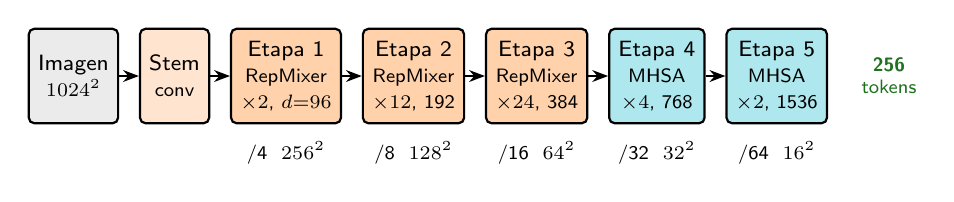
\begin{tikzpicture}[node distance=2.5mm]
  \node[blk, fill=black!8, minimum height=12mm] (in) {Imagen\\\scriptsize $1024^2$};
  \node[blk, fill=cConv!20, right=of in, minimum height=12mm] (st) {Stem\\\scriptsize conv};
  \node[blk, fill=cConv!35, right=of st, minimum height=12mm] (s1) {Etapa 1\\\scriptsize RepMixer\\\scriptsize $\times2$, $d{=}96$};
  \node[blk, fill=cConv!35, right=of s1, minimum height=12mm] (s2) {Etapa 2\\\scriptsize RepMixer\\\scriptsize $\times12$, 192};
  \node[blk, fill=cConv!35, right=of s2, minimum height=12mm] (s3) {Etapa 3\\\scriptsize RepMixer\\\scriptsize $\times24$, 384};
  \node[blk, fill=cAtt!35, right=of s3, minimum height=12mm] (s4) {Etapa 4\\\scriptsize MHSA\\\scriptsize $\times4$, 768};
  \node[blk, fill=cAtt!35, right=of s4, minimum height=12mm] (s5) {Etapa 5\\\scriptsize MHSA\\\scriptsize $\times2$, 1536};
  \foreach \a/\b in {in/st,st/s1,s1/s2,s2/s3,s3/s4,s4/s5}{\draw[arr] (\a) -- (\b);}
  \foreach \n/\l in {s1/{/4\ \ $256^2$},s2/{/8\ \ $128^2$},s3/{/16\ \ $64^2$},s4/{/32\ \ $32^2$},s5/{/64\ \ $16^2$}}{\node[below=1mm of \n, font=\scriptsize] {\l};}
  \node[right=3mm of s5, font=\scriptsize, align=center, text=cProj!70!black] {\textbf{256}\\tokens};
\end{tikzpicture}
\end{document}
